\chapter{Intelig{\^e}ncia Artificial}

O campo de inteligência artificial data desde o primeiros computadores
criados, porém antes mesmo disso, quando o que se possuía eram apenas
máquinas calculadoras e máquinas de programa armazenado, a ideia de se
possuir um sistema capaz de executar suas funções de forma
automatizada já vivia no imaginário dos programadores e cientistas da
época. O termo IA, segundo \citeonline{khemani2013}, só veio a ser
cunhado de maneira oficial por John McCarthy, organizador do workshop
de Dartmouth, seu projeto em conjunto com outros cientistas e
matemáticos da área da computação que resultou em premissas que viriam
a ser utilizadas utilizadas pelos anos a seguir, e também, a
apresentação daquele que é considerado o primeiro programa de
computador funcional como inteligência artificial foi criado por Allen
Newell, Herbert Simon e J. C. Shaw, o Logic Theorist.

\section{Utilizando Intelig{\^e}ncias Artificiais}

Sistemas Inteligentes são todos aqueles definidos como sistemas
formais ou informais utilizados para obter dados e interpretá-los
aplicando tecnologias de Inteligência Artificial (IA) e Business
Intelligence (BI), fornecendo resultados como base para ações
\cite{sharda2017}. Estes sistemas podem ser considerados especialistas
por definição, pois sua base de dados provém de dados abastecidos por
um especialista de determinada área, com seu conhecimento armazenado,
o sistema consegue emular a tomada de decisão de um profissional
inferindo um resultado arbitrário. Ao mesmo tempo que essa é uma
solução interessante para diversas aplicações do mercado, sistemas
especialistas são pouco versáteis por geralmente não terem a
capacidade de gerar resultados fora do universo que já conhecem, os
limitando para simples Inteligências Artificiais.

De acordo com o diagrama da \autoref{fig_euler}, dentro dos escopos dos sistemas
de Inteligência Artificial, aqueles que resolvem tarefas complexas
independentemente ou com pouca intervenção humana \cite{russel2020},
se encontram as aplicações de Aprendizado de Máquina (ML), que são
capazes de melhorar seu desempenho baseando-se numa alteração de seu
modelo analítico e classificando os resultados, fazendo com que
futuras iterações da execução do sistema sejam influenciadas, criando
assim uma “inteligência própria”. O Deep Learning é uma metodologia
mais recente da qual utiliza de padrões de ML e os associa com padrões
biológicos humanos, como a ativação de neurônios simulada por uma rede
neural computacional, explorada adiante, esta metodologia utiliza de
funções mais complexas como convoluções e múltiplas ativações de um
neurônio \cite{janiesch2021} e geralmente possui uma vantagem em
relação à seu supertipo na resolução de problemas de reconhecimento de
placas ou de voz, por conseguirem encontrar padrões nos dados de
entrada dentro da própria tarefa sendo executada.

\begin{figure}[htb]
  \centering
  \caption{\label{fig_euler}Diagrama de Euler da rela{\c c}{\~a}o entre AI, ML e DL.}
  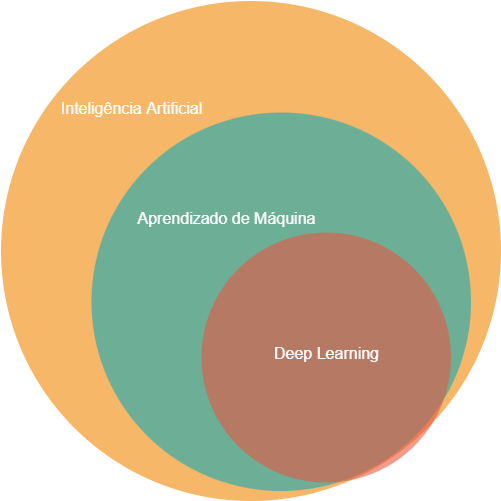
\includegraphics[width=0.7\textwidth]{images/ai-euler.png}
  \legend{
    Fonte: Autoria pr{\'o}pria.
  }
\end{figure}

\section{Estruturando um Problema}

Para se imaginar uma aplicação a inteligências artificiais, primeiro
se faz necessário postular qual é o problema a ser resolvido e quais
os passos a serem tomados que possibilitam o alcance de resultados
satisfatórios. Em um exemplo prático, é possível imaginar um viajante,
que sem qualquer instrução prévia deseja alcançar a cidade de São
Paulo partindo de Sorocaba em no máximo duas horas de viagem, o
objetivo neste caso é claro e se dá em alcançar a cidade de destino
dentro do período de tempo determinado, qualquer outro resultado é
visto como insatisfatório.

Analisando como fazer com que este objetivo seja atingido, é possível
que a instruções o sejam dadas através de movimentos que o carro deve
realizar, como seguir em frente ou virar à esquerda, mas pelo tamanho
do problema proposto, a quantidade de instruções a serem dadas
alcançariam um nível de complexidade muito alto além de serem muito
amplas quanto à quantidade. Estas instruções podem vir a ser
simplificadas realizando uma diminuição em seu escopo, sendo os
possíveis passos deste viajante chegar a cidades vizinhas próximas.

Seus passos então seriam alcançar a cidade de Votorantim, Alumínio ou
Araçoiaba da Serra, cada um adicionando um tempo referente a seu
trajeto, por exemplo, de início ele não saberá qual dessas cidades
possui a melhor rota ou a sequer possibilidade de levá-lo a São Paulo,
como nenhuma destas rotas o faz de fato chegar ao objetivo final, cabe
à aleatoriedade definir se a escolha sendo feita de fato é a melhor
aplicável ou não, adicionando uma camada de incerteza. Tratando-se de
modelos computacionais, existem métodos a serem discutidos a seguir
que pesarão na tomada de decisão.

Dentre os fatores deste problema estruturado, o viajante assume um
ambiente observável, pois este sempre sabe onde está inclusive caso
tenha alcançado seu objetivo no tempo necessário, o ambiente também
pode ser considerado discreto, pois a quantidade de cidades que
delimitam Sorocaba e qualquer outra dentro do trajeto é finita. E o
resultado é sempre determinístico, com uma resposta de destino
alcançado a tempo ou não.

Fazendo um breve paralelo com um algoritmo que viesse a executar este
problema, a entrada de dados seria dada pela posição inicial do
viajante, e dadas as possíveis cidades que este pode seguir, um
retorno seria dado de uma nova lista de cidades com o tempo percorrido
até então, a cada novo passo uma verificação se o objetivo foi
alcançado seria feita, sendo esta a condição de parada em caso de
sucesso ou falha por tempo limite atingido.


\section{Aprendizado de M{\'a}quina}

``Aprendizado'' pode ser definido como processo por meio do qual uma
nova informação é incorporada à estrutura cognitiva do indivíduo, por
se relacionar a um aspecto relevante dessa estrutura. Esse novo
conteúdo poderá modificar aquele já existente, dando-lhe outros
significados \cite{michaelis2022}. Tais características supracitadas
quando implementadas no universo computacional recebem o nome de
Aprendizado de Máquina.

O termo Aprendizado de Máquina foi criado por Arthur Samuel, da IBM,
em 1962 após o desenvolvimento de um algoritmo capaz de vencer um
humano durante uma partida de damas. Comparado ao que pode ser feito
hoje, esse feito quase parece trivial, mas é considerado um marco
importante no campo da inteligência artificial \cite{ibm2022}.
Aprendizado de Máquina consiste em utilizar dados de diferentes fontes
e tipos, e, através de algoritmos baseados em métodos e modelos
matemáticos, executar diferentes tarefas de maneira similar a um ser
humano, fazendo classificações ou predições das situações em que se
encontra inserido.  Os dados necessários para o treinamento de um
modelo de Aprendizado de Máquina podem ser organizados e classificados
previamente através de processos de refinamentos de dados ou dados não
rotulados, apresentados ao modelo de maneira dispersa e não
especificada. A escolha de como tais dados serão utilizados varia de
acordo com o algoritmo e método de treino escolhidos.

Os tipos de treinamento de um modelo de Aprendizado de Máquina podem
ser divididos em três grandes grupos de técnicas classificatórias
primárias, sendo elas: supervisionado, não supervisionado e semi
supervisionado.

Supervisionado: De acordo com \citeonline{miller2014}, aprendizado
supervisionado é uma simples formalização da ideia de aprender através
de exemplos. Nessa técnica, os dados fornecidos ao modelo devem passar
por um tratamento prévio para normalização e organização. Junto a
isso, os dados são separados em treino e teste. Os de treino são
utilizados para ensinar o modelo, já os de teste são utilizados para
verificar a eficácia do aprendizado, comparando o resultado dado pelo
modelo com o resultado já conhecido para aquela combinação de
valores. Por exemplo, para predizer se vai ou não chover com base no
clima, é necessário que o algoritmo tenha uma larga base de dados
sobre a situação meteorológica de dias que choveram e de dias que não
choveram, separando a base em treino e teste e então iniciar o
processo de aprendizado, verificando a eficácia durante o processo
para, então, ao atingir uma boa capacidade preditiva seja possível
utilizar o modelo com dados abstraídos de situações reais.

Não supervisionado: Os algoritmos que utilizam o aprendizado não
supervisionado recebem os dados de maneira não necessariamente
tratados e não rotulados, sem possuir um resultado específico para uma
dada combinação de dados. Esse tipo de aprendizado propicia o
descobrimento de padrões, sendo possível os categorizar sem a
necessidade de análise e intervenção humana. O objetivo do aprendizado
não supervisionado é melhorar o desempenho de tarefas supervisionadas
quando não se possui uma grande quantidade de dados
\cite{sutskever2015}. Essa habilidade de descobrir semelhanças e
diferenças entre utilizando diferentes tipos de dados permite que o
aprendizado não supervisionado possa ser utilizado em reconhecimento
de imagem e segmentação de consumidores, onde é possível caracterizar
tendências de compra com base na maneira com que um grupo de usuários
utiliza as redes sociais, por exemplo.

Semi supervisionado: Nesse modelo, o algoritmo utiliza um meio termo
entre supervisionado e não supervisionado. Durante o treinamento, ele
usa um conjunto de dados rotulados menores para orientar a
classificação e a extração de recursos de um conjunto de dados maior e
não rotulado \cite{uibm2022}. Com isso é possível auxiliar o
descobrimento de diferentes padrões e os classificar baseado no
aprendizado previamente realizado com dados tratados.

\section{Aprendizado por reforco}

O Aprendizado de refor{\c c}o se trata se uma subcategoria de
aprendizado de m{\'a}quina que, de forma sumarizada, mapeia situa{\c
  c}{\~o}es a a{\c c}oes de forma a maximizar uma recompensa
num{\'e}rica. O aprendiz n{\~a}o {\'e} auxiliado em que a{\c c}{\~o}es
tomar, mas deve descobrir quais a{\c c}{\~o}es rendem mais recompensas
ao experiment{\'a}-las \cite{kaelbling1996}. Esse m{\'e}todo
explorat{\'o}rio faz contraste com m{\'e}todos de aprendizado
\textit{supervisionados}, em que o algoritmo recebe a informa{\c
  c}{\~a}o ``correta'' e tenta se aproximar ao m{\'a}ximo dessa
solu{\c c}{\~a}o conhecida; e tamb{\'e}m com os m{\'e}todos n{\~a}o
supervisionados, que utilizam m{\'e}todos de associa{\c c}{\~a}o e
\textit{clustering} para tomar suas decis{\~o}es. A
\autoref{fig_learnings} ilustra as rela{\c c}{\~o}es e principais
diferen{\c c}as entre esses m{\'e}todos.

\begin{figure}[htb]
  \centering
  \caption{\label{fig_learnings}Tabela com classifica{\c c}{\~o}es dos diferentes m{\'e}todos de aprendizado de m{\'a}quina.}
  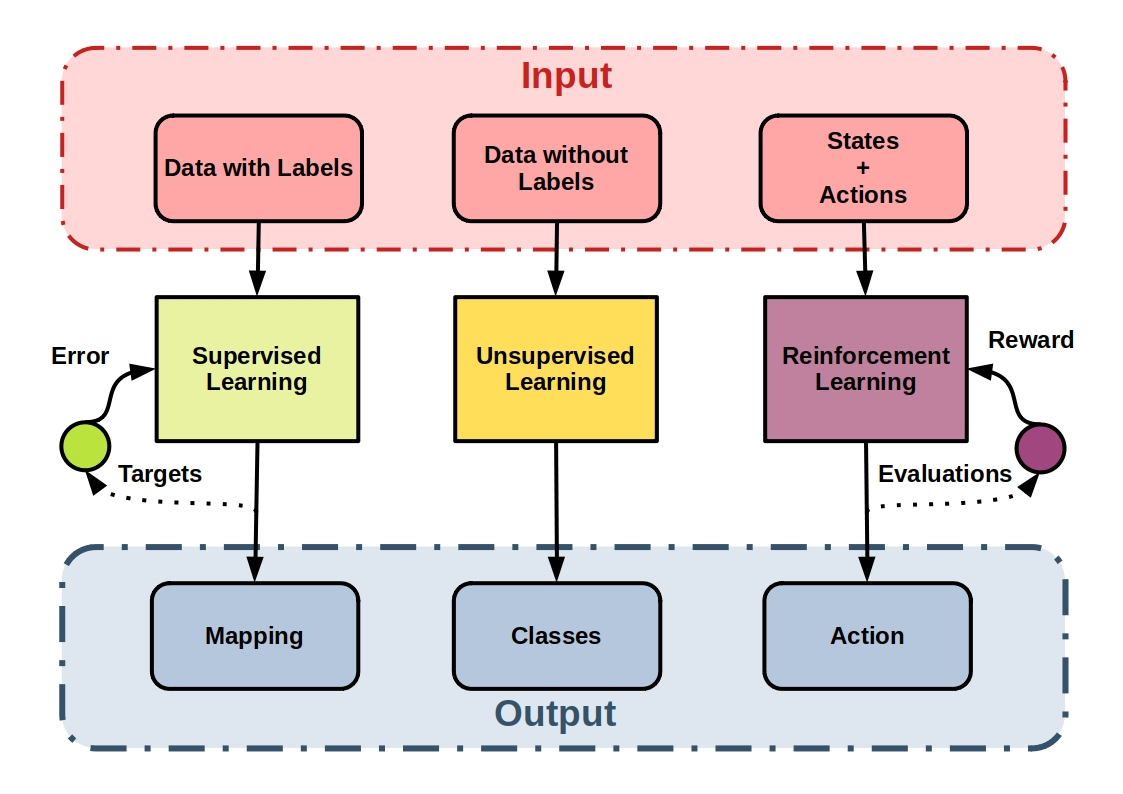
\includegraphics[width=0.7\textwidth]{images/unsupervised_supervised_reinforcement.jpeg}
  \legend{
    \protect\footnotemark
    Dispon{\'i}vel em: \url{https://starship-knowledge.com}. Acesso em: 4 Set. 2022.
  }
\end{figure}

\footnotetext{Imagem retirada de: \url{https://starship-knowledge.com/supervised-vs-unsupervised-vs-reinforcement}}


Esse tipo de aprendizado facilita ou at{\'e} possibilita experimentos
em que outros m{\'e}todos teriam muita dificuldade ou aumentariam a
complexidade do problema significativamente.
\citeonline{sutton2018reinforcement} indica que esse campo de estudo
tem atra{\'i}do cada vez mais interesse nas comunidades de IA e ML,
pelo seu modo de programar agentes por recompensas e puni{\c c}{\~o}es
atrav{\'e}s de tentativa e erro e sem precisar indicar \textit{como} o
problema deve ser resolvido.

Uma das principais aplica{\c c}{\~o}es de aprendizado por refor{\c c}o
se faz em problemas no espa{\c c}o f{\'i}sico, em que se recebe uma
quantidade grande de dados e que a rela{\c c}{\~a}o entre tais dados e
a a{\c c}{\~a}o ou resultado se fazem dif{\'i}ceis por meios
matem{\'a}ticos. Enquanto esses algor{\'i}tmos performam muito bem na
resolu{\c c}{\~a}o dos problemas, o processo de treinamento no mundo
real pode ser extremamente custoso e demorado. Nestes casos, simula{\c
  c}{\~o}es (contanto que sejam pr{\'o}ximas o suficiente da
realidade) podem trazer uma atraente alternativa para simplificar o
treinamento de um modelo complexo \cite{Rao_2020_CVPR}.

\section{NEAT}

\lipsum[6-8]
